\chapter{Application layer}\label{sec:application_layer}

Previous chapters of this specification define a set of basic concepts that are the foundation of the protocol:
they allow one to define data structures and exchange them over the bus in a robust and deterministic manner.
This chapter is focused on higher-level concepts: rules, conventions, and standard functions that are to be
respected by applications utilizing UAVCAN to maximize cross-vendor compatibility, avoid ambiguities, and
prevent some common design pitfalls.

The rules, conventions, and standard functions defined in this chapter are designed to be an acceptable middle
ground for any sensible aerospace or robotic system.
UAVCAN does not attempt to favor any particular domain or kind of systems among targeted applications.

Unless stated otherwise, all of the high-level functions described in this chapter are optional,
meaning that they do not necessarily have to be supported or implemented for an application or system to be
UAVCAN-compliant.
Excepting a very few mandatory functions and rules, users of UAVCAN are allowed to pick only those
that are needed and suitable for their applications.

If a designer choses to deviate from the rules and conventions presented in this chapter,
every such deviation should be explicitly documented.

\clearpage\section{Application-level conventions}\label{sec:application_conventions}

This section describes a set of high-level conventions designed to enhance compatibility
of applications leveraging UAVCAN.
The conventions described here are not mandatory to follow;
however, every deviation should be justified and documented.

\subsection{Node identifier distribution}

An overview of related concepts is provided in chapter~\ref{sec:basic}.

Valid values of node-ID range from 0 up to a transport-specific upper boundary
which is guaranteed to be above 127 for any transport.

The two uppermost node-ID values are reserved for diagnostic and debugging tools;
these node-ID values should not be used in fielded systems.

\subsection{Timing constraints}

\subsubsection{Recommended message publication timing constraints}

Generally, it is recommended to abort a message transmission if it cannot be completed in 1 second.

It is expected that high-frequency high-priority messages may opt for lower timeout values,
whereas low-priority delayable data may opt for higher timeout values to account for network congestion.
Refer to section~\ref{sec:transport_transfer_priority} on transfer prioritization.

\subsubsection{Recommended service invocation timing constraints}

It is recommended to abort a service transfer transmission if it cannot be completed in 1 second.
It is recommended to stop waiting for a service response if it could not be received in the same amount of time;
upon reaching this condition, the service request operation should be considered unsuccessful.

If the server uses a significant part of the timeout period to process the request,
the client might drop the request before receiving the response.
It is recommended to ensure that the server will be able to process any request in less than 0.5 seconds.

\subsection{Coordinate frames}

UAVCAN follows the conventions that are widely accepted in relevant applications.
Adherence to the coordinate frame conventions described here maximizes compatibility and
reduces the amount of computations for conversions between incompatible coordinate systems and
representations.
It is recognized, however, that some applications may find the advised conventions unsuitable,
in which case deviations are permitted.
Any such deviations shall be explicitly documented.

All coordinate systems defined in this section are right-handed.
If application-specific coordinate systems are introduced, they should be right-handed as well.

\begin{figure}[hbt]
    \centering
    % The source image is released under CC0, public domain, no attribution required:
    % https://commons.wikimedia.org/wiki/File:ECEF_ENU_Longitude_Latitude_relationships.svg
	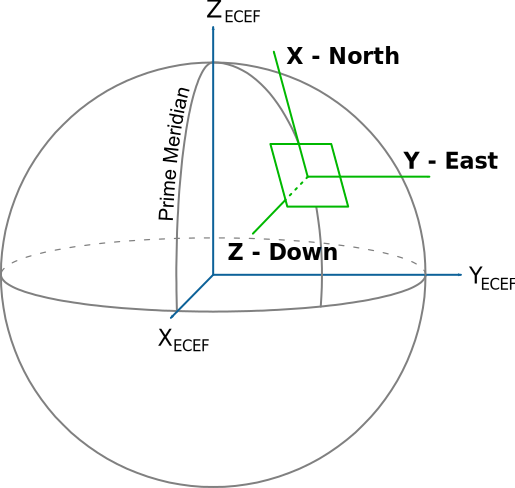
\includegraphics[width=0.45\textwidth]{application/NED_ECEF}
    % The source image is released under CC0, public domain, no attribution required:
    % https://pixabay.com/en/airplane-plane-aircraft-propeller-40374/
    % The final image is drawn by me. The source Inkscape SVG file is located in the same directory.
    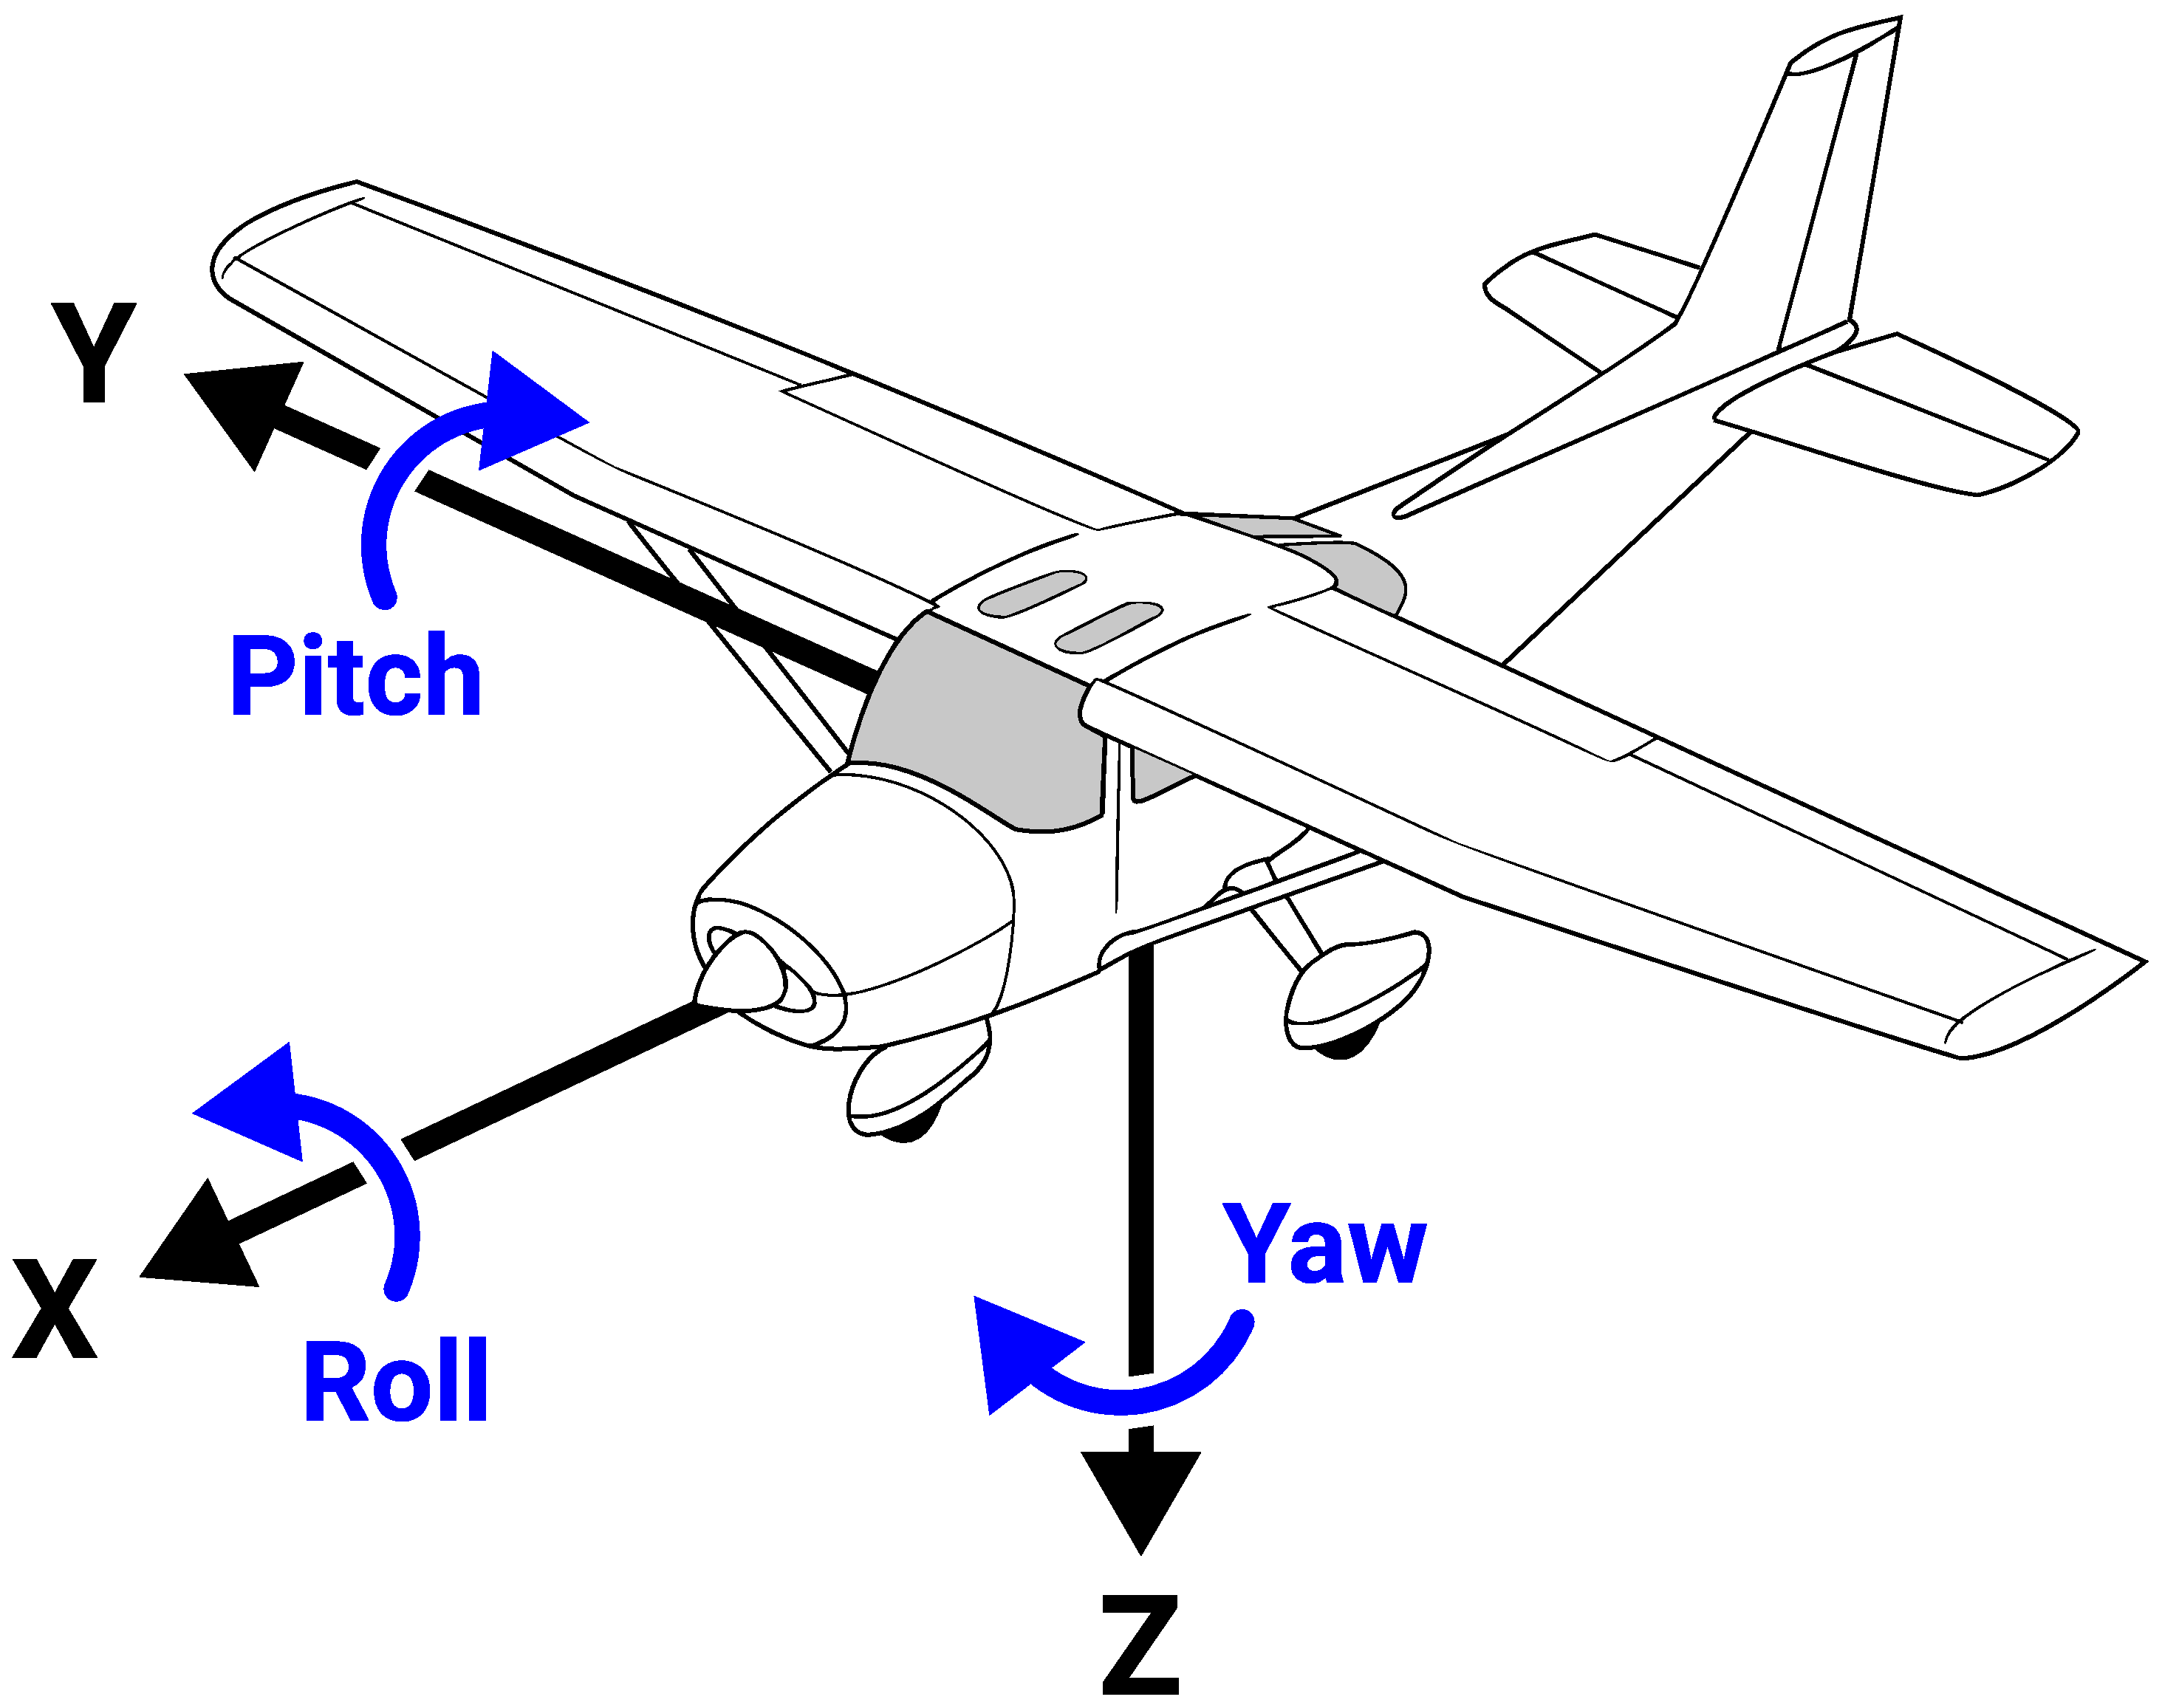
\includegraphics[width=0.45\textwidth]{application/aircraft_principal_axes}
    North-East-Down (NED) frame and body frame conventions. All systems are right-handed.
    \caption{Coordinate frame conventions\label{fig:application_conventions_coordinate_frame}}
\end{figure}

\subsubsection{World frame}

For world fixed frames, the \emph{North-East-Down} (NED) right-handed notation is preferred.
\begin{samepage}
    \begin{description}
        \item[X] --- northward;
        \item[Y] --- eastward;
        \item[Z] --- down.
    \end{description}
\end{samepage}

\subsubsection{Body frame}

In relation to a body, the convention is as defined below, right-handed.
This convention is widely used in aeronautic applications.
\begin{samepage}
    \begin{description}
        \item[X] --- forward;
        \item[Y] --- right;
        \item[Z] --- down.
    \end{description}
\end{samepage}

\subsubsection{Optical frame}

In the case of cameras, the right-handed convention specified below is preferred.
It is widely used in various applications involving computer vision systems.
\begin{samepage}
    \begin{description}
        \item[X] --- right;
        \item[Y] --- down;
        \item[Z] --- towards the scene along the optical axis.
    \end{description}
\end{samepage}

\subsection{Rotation representation}

All applications should represent rotations using quaternions with the elements ordered as follows\footnote{%
    Assuming $w + x\boldsymbol{i} + y\boldsymbol{j} + z\boldsymbol{k}$.
}: W, X, Y, Z.
Other forms of rotation representation should be avoided.

Angular velocities should be represented using the right-handed, fixed-axis (extrinsic) convention:
X (roll), Y (pitch), Z (yaw).

\begin{remark}
    Quaternions are considered to offer the optimal trade-off between bandwidth efficiency,
    computation complexity, and explicitness:
    \begin{itemize}
        \item Euler angles are not self-contained, requiring applications to agree on a particular
              convention beforehand; a convention would be difficult to establish considering different
              demands of various use cases.

        \item Euler angles and fixed axis rotations typically cannot be used for computations directly
              due to angular interpolation issues and singularities; thus, to make use of such
              representations, one often has to convert them to a different form (e.g., quaternion);
              such conversions are computationally heavy.

        \item Rotation matrices are highly redundant.
    \end{itemize}
\end{remark}

\subsection{Matrix representation}

\subsubsection{General}

Matrices should be represented as flat arrays in the row-major order.

\begin{remark}
    $
    \begin{bmatrix}
        x_{11} & x_{12} & x_{13} \\
        x_{21} & x_{22} & x_{23} \\
    \end{bmatrix} \rightarrow \left(x_{11}, x_{12}, x_{13}, x_{21}, x_{22}, x_{23}\right)
    $
\end{remark}

\subsubsection{Square matrices}

There are standard compressed representations of an $n \times n$ square matrix.

An array of size $n^2$ represents a full square matrix.
This is equivalent to the general case reviewed above.

An array of $\frac{(1 + n) n}{2}$ elements represents a symmetric matrix,
where array members represent the elements of the upper-right triangle arranged in the row-major order.
\begin{remark}
    $
    \begin{bmatrix}
        a & b & c \\
        b & d & e \\
        c & e & f \\
    \end{bmatrix} \rightarrow \left(a, b, c, d, e, f\right)
    $

    This form is well-suited for covariance matrix representation.
\end{remark}

An array of $n$ elements represents a diagonal matrix,
where an array member at position $i$ (where $i=1$ for the first element)
represents the matrix element $x_{i, i}$ (where $x_{1, 1}$ is the upper-left element).
\begin{remark}
    $
    \begin{bmatrix}
        a & 0 & 0 \\
        0 & b & 0 \\
        0 & 0 & c \\
    \end{bmatrix} \rightarrow \left(a, b, c\right)
    $
\end{remark}

An array of one element represents a scalar matrix.
\begin{remark}
    $
    \begin{bmatrix}
        a & 0 & 0 \\
        0 & a & 0 \\
        0 & 0 & a \\
    \end{bmatrix} \rightarrow a
    $
\end{remark}

An empty array represents a zero matrix.

\subsubsection{Covariance matrices}

A zero covariance matrix represents an unknown covariance\footnote{%
    As described above, an empty array represents a zero matrix,
    from which follows that an empty array represents unknown covariance.
}.

Infinite error variance means that the associated value is undefined.

\subsection{Physical quantity representation}

\subsubsection{Units}

All units should be SI\footnote{International System of Units.} units (base or derived).
Usage of any other units is strongly discouraged.

When defining data types, fields and constants that represent unscaled quantities in SI units
should not have suffixes indicating the unit, since that would be redundant.

On the other hand, fields and constants that contain quantities in
non-SI units\footnote{E.g., degree Celsius instead of kelvin.}
or scaled SI units\footnote{E.g., microsecond instead of second.}
should be suffixed with the standard abbreviation of the unit\footnote{E.g., kg for kilogram, J for joule.}
and its metric prefix\footnote{E.g., M for mega, n for nano.}
(if any), maintaining the proper letter case of the abbreviation.
In other words, the letter case of the suffix is independent of the letter case of
the attribute it is attached to.

Scaling coefficients should not be chosen arbitrarily;
instead, the choice should be limited to the standard metric prefixes defined by the
International System of Units.

All standard metric prefixes have well-defined abbreviations that are constructed from ASCII characters,
except for one: the micro prefix is abbreviated as a Greek letter ``\textmu{}'' (mu).
When defining data types, ``\textmu{}'' should be replaced with the lowercase Latin letter ``u''.

Irrespective of the suffix, it is recommended to always specify units for every field in the comments.

\begin{remark}
    \begin{minted}{python}
        float16 temperature           # [kelvin] Suffix not needed because an unscaled SI unit is used here.

        uint24 delay_us               # [microsecond] Scaled SI unit, suffix required. Mu replaced with "u".
        uint24 MAX_DELAY_us = 600000  # [microsecond] Notice the letter case.

        float32 kinetic_energy_GJ     # [gigajoule] Notice the letter case.

        float16 estimated_charge_mAh  # [milliampere hour] Scaled non-SI unit. Discouraged, use coulomb.
        float16 MAX_CHARGE_mAh = 1e4  # [milliampere hour] Notice the letter case.
    \end{minted}
\end{remark}

\subsubsection{Enhanced type safety}

In the interest of improving type safety and reducing the possibility of a human error,
it is recommended to avoid reliance on raw scalar types (such as \verb|float32|)
when defining fields containing physical quantities.
Instead, the explicitly typed alternatives defined in the standard DSDL namespace
\DSDLReference{uavcan.si.unit} (also see section~\ref{sec:application_functions_si}) should be used.

\begin{remark}
    \begin{minted}{python}
        float32[4] kinetic_energy                           # [joule] Not recommended.
        uavcan.si.unit.energy.Scalar.1.0[4] kinetic_energy  # This is the recommended practice.
        # Kinetic energy of four bodies.

        float32[3] velocity                                 # [meter/second] Not recommended.
        uavcan.si.unit.velocity.Vector3.1.0                 # This is the recommended practice.
        # 3D velocity vector.
    \end{minted}
\end{remark}

\clearpage\section{Application-level functions}\label{sec:application_level_functions}

This section documents the high-level functionality defined by UAVCAN.
The common high-level functions defined by the specification span across different application domains.
All of the functions defined in this section are optional (not mandatory to implement),
except for the node heartbeat feature (section \ref{sec:application_node_heartbeat}),
which is mandatory for all UAVCAN nodes.

The detailed specifications for each function are provided in the DSDL comments of the data type definitions
they are built upon, whereas this section serves as a high-level overview and index.

\subsection{Node initialization}

UAVCAN does not require that nodes undergo any specific initialization upon connection to the bus ---
a node is free to begin functioning immediately once it is powered up.
The operating mode of the node (such as initialization, normal operation, maintenance, and so on)
is to be reflected via the mandatory heartbeat message described in section \ref{sec:application_node_heartbeat}.

\subsection{Node heartbeat}\label{sec:application_node_heartbeat}

Every non-anonymous UAVCAN node shall report its status and presence by periodically publishing messages of type
\DSDLReference{uavcan.node.Heartbeat} at a fixed rate specified in the message definition using the fixed subject-ID.
Anonymous nodes shall not publish to this subject.

This is the only high-level protocol function that UAVCAN nodes are required to support.
All other data types and application-level functions are optional.

\DSDL{uavcan.node.Heartbeat}

\subsection{Generic node information}

The service \DSDLReference{uavcan.node.GetInfo} can be used to obtain generic information about the node,
such as the structured name of the node (which includes the name of its vendor),
a 128-bit globally unique identifier, the version information about its hardware and software,
version of the UAVCAN specification implemented on the node, and the optional certificate of authenticity.

While the service is, strictly speaking, optional, omitting its support is highly discouraged,
since it is instrumental for network discovery, firmware update, and various maintenance and diagnostic needs.

\DSDL{uavcan.node.GetInfo}

\subsection{Bus data flow monitoring}

The combination of the following three services defined in the namespace \DSDLReference{uavcan.node.port}
(see table \ref{table:dsdl:uavcan.node.port}) enables a highly capable tool of network inspection and monitoring:
\begin{itemize}
    \item \DSDLReference{uavcan.node.port.List} --- designed for obtaining the full set of subjects and services
    implemented by the server node.

    \item \DSDLReference{uavcan.node.port.GetInfo} --- returns the static (unchanging or infrequently changing)
    information about the selected subject or service.

    \item \DSDLReference{uavcan.node.port.GetStatistics} --- returns the transfer event counters of
    the selected subject or service.
\end{itemize}

The first service \verb|List| allows the caller to construct a list of all subjects and services used by the
server node (i.e., the node that the request was sent to).
The second service \verb|GetInfo| allows the caller to map each subject or service to a particular data type,
and understand the role of the server node in relation to said subject or service
(publisher, subscriber, or server).

By comparing the data obtained with the help of these two services from each node on the bus,
the caller can reconstruct the data exchange graph for the entire bus,
thus enabling advanced network monitoring and diagnostics
(assuming that every node on the bus supports the services in question; they are not mandatory).

The last service \verb|GetStatistics| can be used to sample the number of transfers and errors observed
on the specified port.
When invoked periodically, this service allows the caller to observe the real time intensity of data exchange
for each port independently.
In combination with the data exchange graph reconstruction described earlier,
this service allows the caller to build a sophisticated real-time view of the bus.

\DSDL{uavcan.node.port.* --index-only}

\subsection{Network-wide time synchronization}

UAVCAN provides a simple and robust method of time synchronization%
\footnote{The ability to accurately synchronize time between nodes is instrumental for building distributed
real-time data processing systems such as various robotic applications, autopilots, autonomous driving solutions,
and so on.} that is built upon the work
``Implementing a Distributed High-Resolution Real-Time Clock using the CAN-Bus''
published by M.~Gergeleit and H.~Streich%
\footnote{Proceedings of the 1st international CAN-Conference 94, Mainz,
13.-14. Sep. 1994, CAN in Automation e.V., Erlangen.}.
The detailed specification of the time synchronization algorithm is provided in the documentation
for the message type \DSDLReference{uavcan.time.Synchronization}.

\DSDLReference{uavcan.time.GetSynchronizationMasterInfo} provides nodes with information about
the currently used time system and related data like the number of leap seconds added.

Redundant time synchronization masters are supported for the benefit of high-reliability applications.

\begin{remark}
    Time synchronization with explicit sensor feed timestamping should be preferred over inferior alternatives
    such as sensor lag reporting that are sometimes found in simpler systems because such alternatives
    are difficult to scale and they do not account for the delays introduced by communication interfaces.

    It is the duty of every node that publishes timestamped data to account for its own internal delays;
    for example, if the data latency of a local sensor is known,
    it needs to be accounted for in the reported timestamp value.
\end{remark}

\DSDL{uavcan.time.* --index-only}

\subsection{Primitive types and physical quantities}

The namespaces \DSDLReference{uavcan.si} and \DSDLReference{uavcan.primitive}
included in the standard data type set are designed to provide a generic and flexible
method of real-time data exchange. However, these are not bandwidth-efficient.

Generally, applications where the bus bandwidth and latency are important should minimize their reliance
on these generic data types and favor more specialized types instead that are custom-designed for their
particular use cases; e.g., vendor-specific types or application-specific types, either
designed in-house, published by third parties\footnote{As long as the license permits.}, or supplied by
vendors of COTS equipment used in the application.

Vendors of COTS equipment are recommended to ensure that some minimal functionality is available
via these generic types without reliance on their vendor-specific types (if there are any).
This is important for reusability, because some of the systems where such COTS nodes are
to be integrated may not be able to easily support vendor-specific types.

\subsubsection{SI namespace}\label{sec:application_si}

The \verb|si| namespace is named after the International System of Units (SI).
The namespace contains a collection of scalar and vector value types that describe most commonly used
physical quantities in SI; for example, velocity, mass, energy, angle, and time.
The objective of these types is to permit construction of arbitrarily complex distributed control systems without
reliance on any particular vendor-specific data types.

The namespace \DSDLReference{uavcan.si.unit} contains basic units that can be used as type-safe wrappers
over \verb|float32| and other scalar and array types.

The namespace \DSDLReference{uavcan.si.sample} contains time-stamped versions of the above,
where the timestamp field is always located at the end in order to make the time-stamped types
structural sub-types of the non-timestamped ones.
The structural sub-typing enhances interoperability.

Each message type defined in the namespace \verb|uavcan.si.sample| contains a timestamp field of type
\DSDLReference{uavcan.time.SynchronizedTimestamp}.
Every emitted message should be timestamped in order to allow subscribers to identify which of the messages
relate to the same event or to the same instant.
Messages that are emitted in bulk in relation to the same event or the same instant should contain
exactly the same value of the timestamp to simplify the task of timestamp matching for the subscribers.

The exact strategy of matching related messages by timestamp employed by subscribers is entirely
implementation-defined.
The specification does not concern itself with this matter because it is expected that different applications
will opt for different design trade-offs and different tactics to suit their constraints.
Such diversity is not harmful, because its effects are always confined to the local node and cannot affect
operation of other nodes or their compatibility.

The tables \ref{table:dsdl:uavcan.si.unit} and \ref{table:dsdl:uavcan.si.sample}
provide a high-level overview of the SI namespace.
Please follow the references for details.

\DSDL{uavcan.si.unit.* --index-only}

\DSDL{uavcan.si.sample.* --index-only}

\subsubsection{Primitive namespace}

The primitive namespace contains a collection of primitive types:
integer types, floating point types, bit flag, string, raw block of bytes, and an empty value.
Integer, floating point, and bit flag types are available in two categories: scalar and array;
the latter are limited so that their serialized representation is never larger than 257 bytes.

The primitive types are designed to complement the SI namespace with an even simpler set of basic types
that do not make any assumptions about the meaning of the data they describe.
The primitive types provide a very high degree of flexibility, but due to their lack of semantic information,
their use carries the risk of creating suboptimal interfaces that are difficult to use, validate, and scale.

Normally, the use of primitive types should be limited to very basic vendor-neutral interfaces for COTS
equipment and software, debug and diagnostic purposes, and whenever there is a need to exchange data the
type of which cannot be determined statically.\footnote{An example of the latter use case is the register protocol
described in section \ref{sec:application_register_interface}.}

The table \ref{table:dsdl:uavcan.primitive} provides a high-level overview of the primitive namespace.
Please follow the references for details.

\DSDL{uavcan.primitive.* --index-only}

\subsection{Remote file system interface}\label{sec:application_file_system}

The set of standard data types contains a collection of services for manipulation of remote file systems
(namespace \DSDLReference{uavcan.file}, see the table \ref{table:dsdl:uavcan.file}).
All basic file system operations are supported, including file reading and writing,
directory listing, metadata retrieval (size, modification time, etc.), moving, renaming, creating, and deleting.

The set of supported operations may be extended in future versions of the protocol.

Implementers of file servers are strongly advised to always support services \verb|Read| and \verb|GetInfo|,
as that allows clients to make assumptions about the minimal degree of available service.
If write operations are required, all of the defined services should be supported.

\DSDL{uavcan.file.* --index-only}

\subsection{Generic node commands}\label{sec:application_generic_node_commands}

Commonly used node-level application-agnostic auxiliary commands
(such as: restart, power off, factory reset, emergency stop, etc.)
are supported via the standard service \DSDLReference{uavcan.node.ExecuteCommand}.
The service also allows vendors to define vendor-specific commands alongside the standard ones.

It is recommended to support this service in all nodes.

\subsection{Node software update}

A simple software\footnote{Or firmware -- UAVCAN does not distinguish between the two.}
update protocol is defined on top of the remote file system interface (section \ref{sec:application_file_system})
and the generic node commands (section \ref{sec:application_generic_node_commands}).

The software update process involves the following data types:

\begin{itemize}
    \item \DSDLReference{uavcan.node.ExecuteCommand} -- used to initiate the software update process.
    \item \DSDLReference{uavcan.file.Read} -- used to transfer the software image file(s)
          from the file server to the updated node.
\end{itemize}

The software update protocol logic is described in detail in the documentation for the data type
\DSDLReference{uavcan.node.ExecuteCommand}.
The protocol is considered simple enough to be usable in embedded bootloaders with
small memory-constrained microcontrollers.

\subsection{Register interface}\label{sec:application_register_interface}

UAVCAN defines the concept of \emph{named register} -- a scalar, vector, or string value with an associated
human-readable name that is stored on a UAVCAN node locally and is accessible via
UAVCAN\footnote{And, possibly, other interfaces.} for reading and/or modification
by other nodes on the bus.

Named registers are designed to serve the following purposes:
\begin{description}
    \item[Node configuration parameter management] --- Named registers can be used to expose persistently stored
          values that define behaviors of the local node.

    \item[Diagnostics and monitoring] --- Named registers can be used to expose internal states (variables) of
          the node's decision-making and data processing logic (implemented in software or hardware) to provide
          insights about its inner processes.

    \item[Advanced node information reporting] --- Named registers can store any invariants provided by the vendor,
          such as calibration coefficients or unique identifiers.

    \item[Special functions] --- Non-persistent named registers can be used to trigger specific behaviors or
          start predefined operations when written.

    \item[Advanced debugging] --- Registers following a specific naming pattern can be used to provide direct read
          and write access to the local node's application software to facilitate in-depth debugging and monitoring.
\end{description}

The register protocol rests upon two service types defined in the namespace \DSDLReference{uavcan.register};
the namespace index is shown in the table \ref{table:dsdl:uavcan.register}.
Data types supported by the register protocol are defined in the nested data structure
\DSDLReference{uavcan.register.Value}.

The UAVCAN specification defines several standard naming patterns to facilitate cross-vendor compatibility
and provide a framework of common basic functionality.

\DSDL{uavcan.register.* --index-only}

\subsection{Diagnostics and event logging}

The message type \DSDLReference{uavcan.diagnostic.Record} is designed to facilitate emission of
human-readable diagnostic messages and event logging,
both for the needs of real-time display\footnote{E.g., messages displayed to a human operator/pilot in real time.}
and for long-term storage\footnote{E.g., flight data recording.}.

\subsection{Plug-and-play nodes}

Every UAVCAN node shall have a node-ID that is unique within the network (excepting anonymous nodes).
Normally, such identifiers are assigned by the network designer, integrator, some automatic external tool,
or another entity that is external to the network.
However, there exist circumstances where such manual assignment is either difficult or undesirable.

Nodes that can join any UAVCAN network automatically without any prior manual configuration
are called \emph{plug-and-play nodes} (or \emph{PnP nodes} for brevity).

Plug-and-play nodes automatically obtain a node-ID and deduce all necessary parameters of the physical layer
such as the bit rate.

UAVCAN defines an automatic node-ID allocation protocol that is built on top of the data types defined in the
namespace \DSDLReference{uavcan.pnp} (where \emph{pnp} stands for ``plug-and-play'')
(see table \ref{table:dsdl:uavcan.pnp}).
The protocol is described in the documentation for the data type \DSDLReference{uavcan.pnp.NodeIDAllocationData}.

The plug-and-play node-ID allocation protocol relies on anonymous messages reviewed in section
\ref{sec:transport_route_specifier}.
Remember that the plug-and-play feature is entirely optional and it is expected that applications where a
high degree of determinism and robustness is expected are unlikely to benefit from it.

This feature derives from the work
``In search of an understandable consensus algorithm''%
\footnote{Proceedings of USENIX Annual Technical Conference, p. 305-320, 2014.}
by Diego Ongaro and John Ousterhout.

\DSDL{uavcan.pnp.* --index-only}

\subsection{Internet/LAN forwarding interface}

Data types defined in the namespace \DSDLReference{uavcan.internet} (see table \ref{table:dsdl:uavcan.internet})
are designed for establishing robust direct connectivity between local UAVCAN nodes and hosts on the Internet
or on a local area network (LAN) by means of so called \emph{modem nodes}%
\footnote{Normally, a modem node would be implemented using on-board cellular, radio frequency,
or satellite communication hardware.}
(possibly redundant).

This basic support for world-wide communication provided at the protocol level allows any component
of a vehicle equipped with modem nodes to reach external resources or exchange arbitrary data globally
without dependency on application-specific means of communication%
\footnote{Information security and other security-related concerns are outside of the scope of this specification.}.

The set of supported Internet/LAN protocols may be extended in future revisions of the specification.

\begin{remark}
    Some of the major applications for this feature are as follows:
    \begin{enumerate}
        \item Direct telemetry transmission from UAVCAN nodes to a remote data collection server.
        \item Implementation of remote API for on-board equipment (e.g., web interface).
        \item Reception of real-time correction data streams (e.g., RTCM RC-104)
              for precise positioning applications.
        \item Automatic upgrades directly from the vendor's Internet resources.
    \end{enumerate}
\end{remark}

\DSDL{uavcan.internet.* --index-only}

\subsection{Meta-transport}

Data types defined in the namespace \DSDLReference{uavcan.metatransport}
(see table \ref{table:dsdl:uavcan.metatransport})
are designed for tunneling transport frames\footnote{Section \ref{sec:transport_model}.}
over UAVCAN subjects,
as well as logging UAVCAN traffic in the form of serialized UAVCAN message objects.

\DSDL{uavcan.metatransport.* --index-only}

